\documentclass{article}
\author{Alejandro Zubiri}
\date{Thu Oct 10 2024}
\title{Límite y Continuidad}

\usepackage{graphicx}
\usepackage{amsmath, amsthm, physics, amsfonts}

\newtheorem{sandwich}{Teorema}

\graphicspath{{../images/}}

\newtheorem{unicidad}{Teorema}

\begin{document}
\maketitle
\tableofcontents
\pagebreak
\section{Definición de límite}
\begin{equation}
    \begin{split}
        \lim_{x \to a} f(x)=l
    \end{split}
\end{equation}
La función $f$ tiende hacia el valor $l$ a medida que $x$ se aproxima al valor $a$.\\
\begin{equation}
    \begin{split}
        \forall \varepsilon>0, \exists \delta > 0 : \forall x, 0<|x-a|<\delta\Rightarrow |f(x)-l|<\varepsilon
    \end{split}
\end{equation}
Esto significa que el límite de $f$ cuando $x$ se acerca al valor $a$ es $l$ si, para cualquier valor real $\varepsilon>0$,
existe otro valor $\delta>0$ tal que la distancia entre $x$ y $a$ $(|x-a|)$ es menor que $\delta$, y la distancia
entre $f$ y $l$ $(|f(x)-l|)$ es menor que $\varepsilon$.
\section{Límites laterales}
\subsection{Límite lateral por la izquierda}
\begin{equation}
    \begin{split}
        \lim_{x \to a^{-}}= l^{-}
    \end{split}
\end{equation}
Se cumple si dado un valor real $\varepsilon>0,\exists \delta>0$ tal que si $a-\delta<x<a\Rightarrow |f(x)-l^-|<\varepsilon$.\\
\begin{center}
    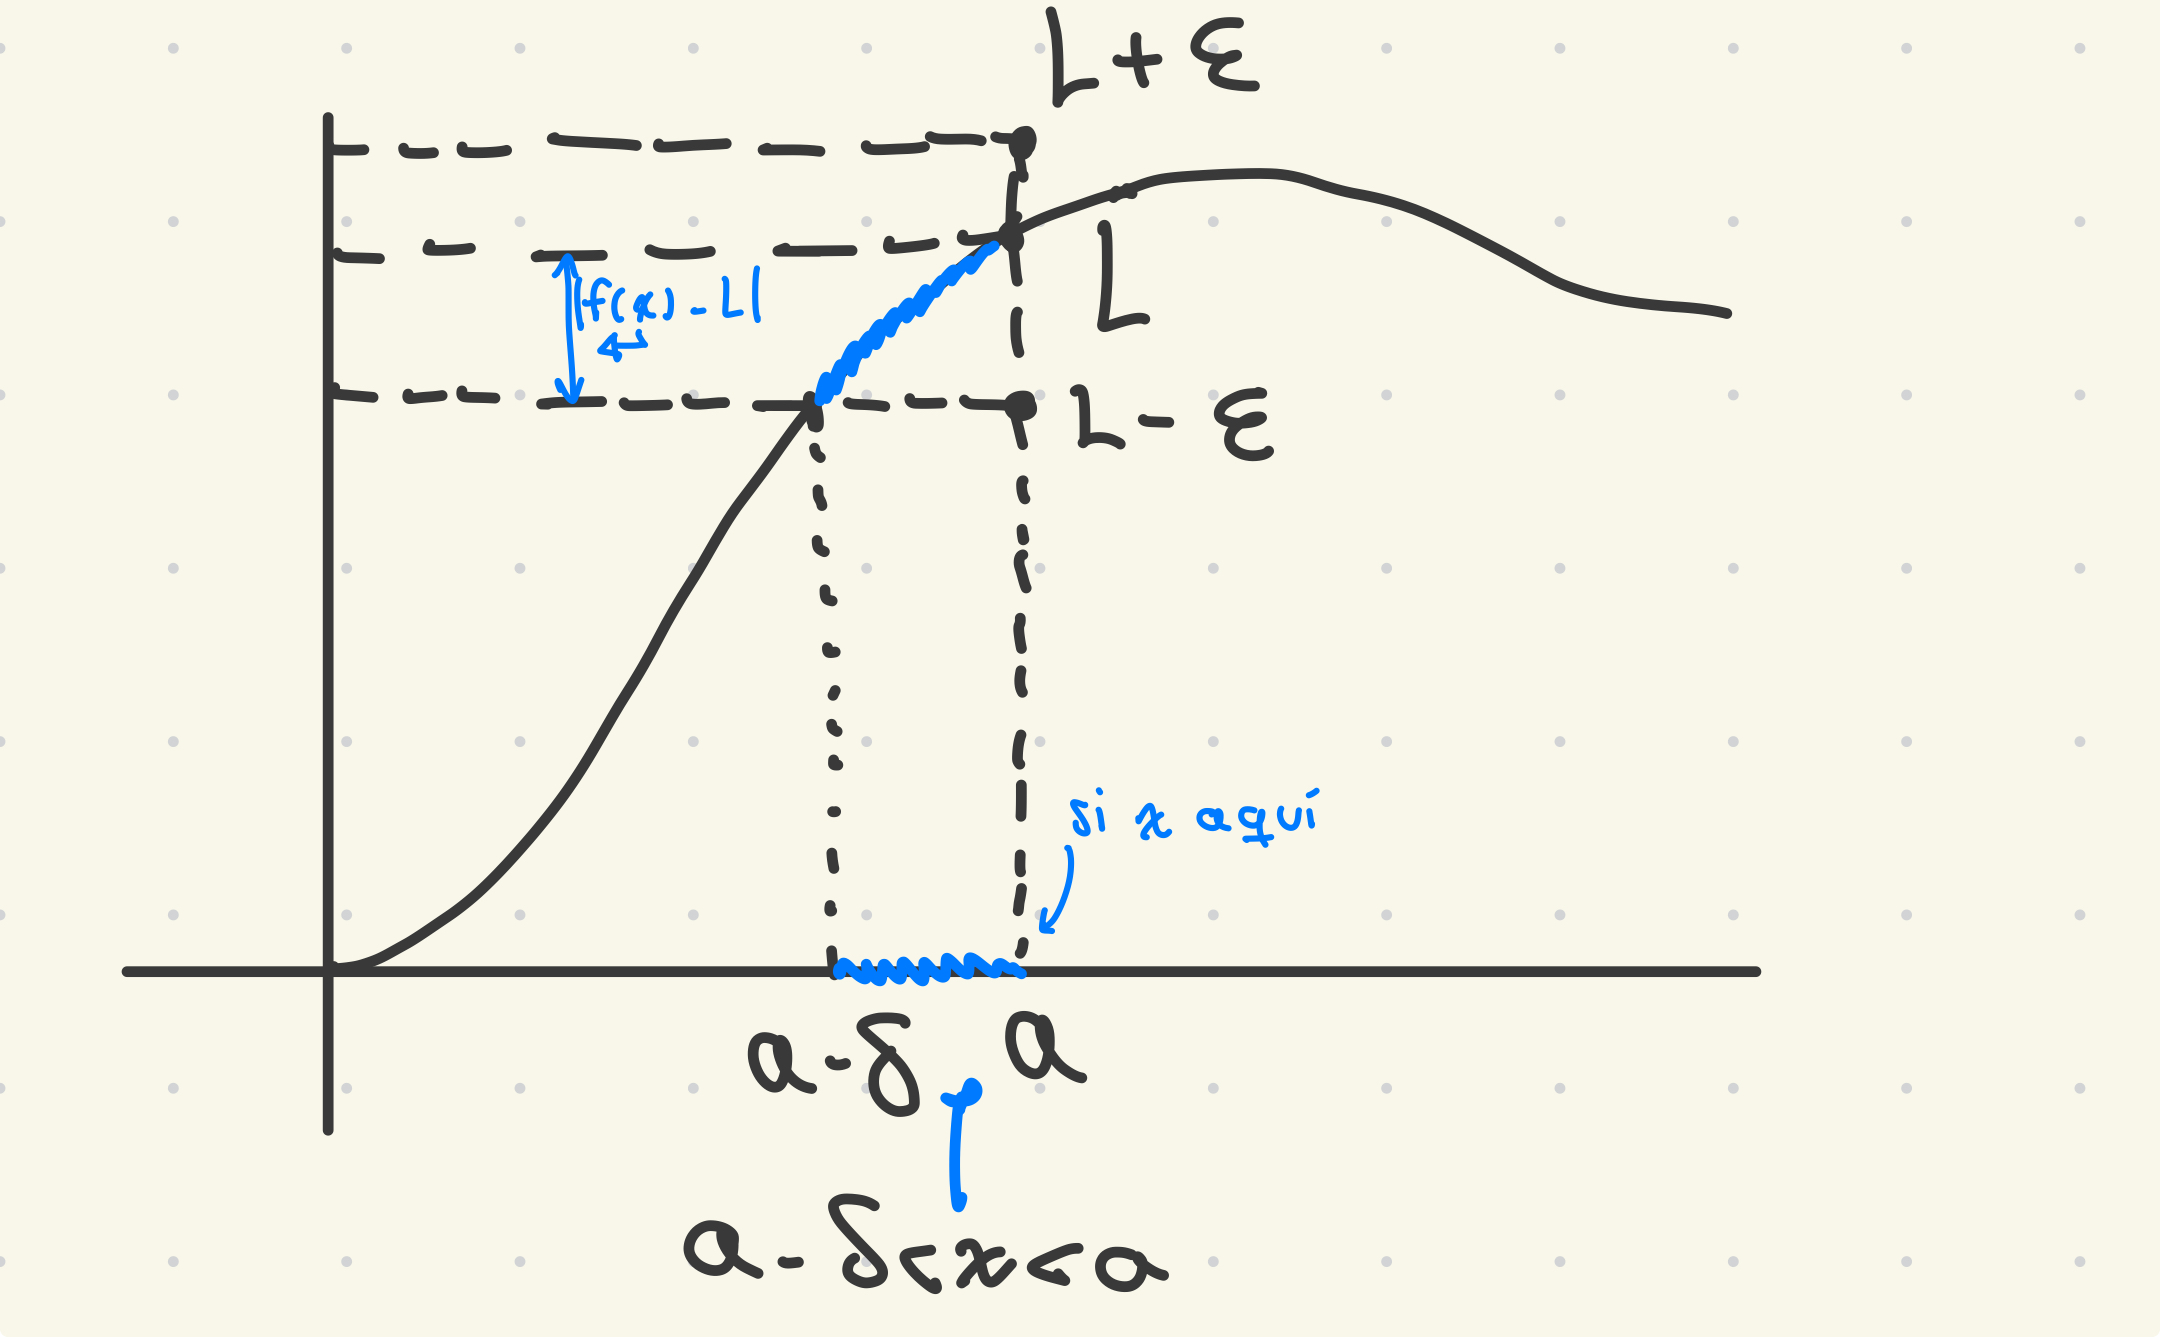
\includegraphics[height =100px]{limIzquierda.jpg}
\end{center}
\subsection{Límite lateral por la derecha}
\begin{equation}
    \begin{split}
        \lim_{x \to a^+}=l^{+}
    \end{split}
\end{equation}
Se cumple si dado $\varepsilon>0, \exists \delta > 0$ tal que si $a<x<a+\delta \Rightarrow |f(x)-l^+|<\varepsilon$.\\
\begin{center}
    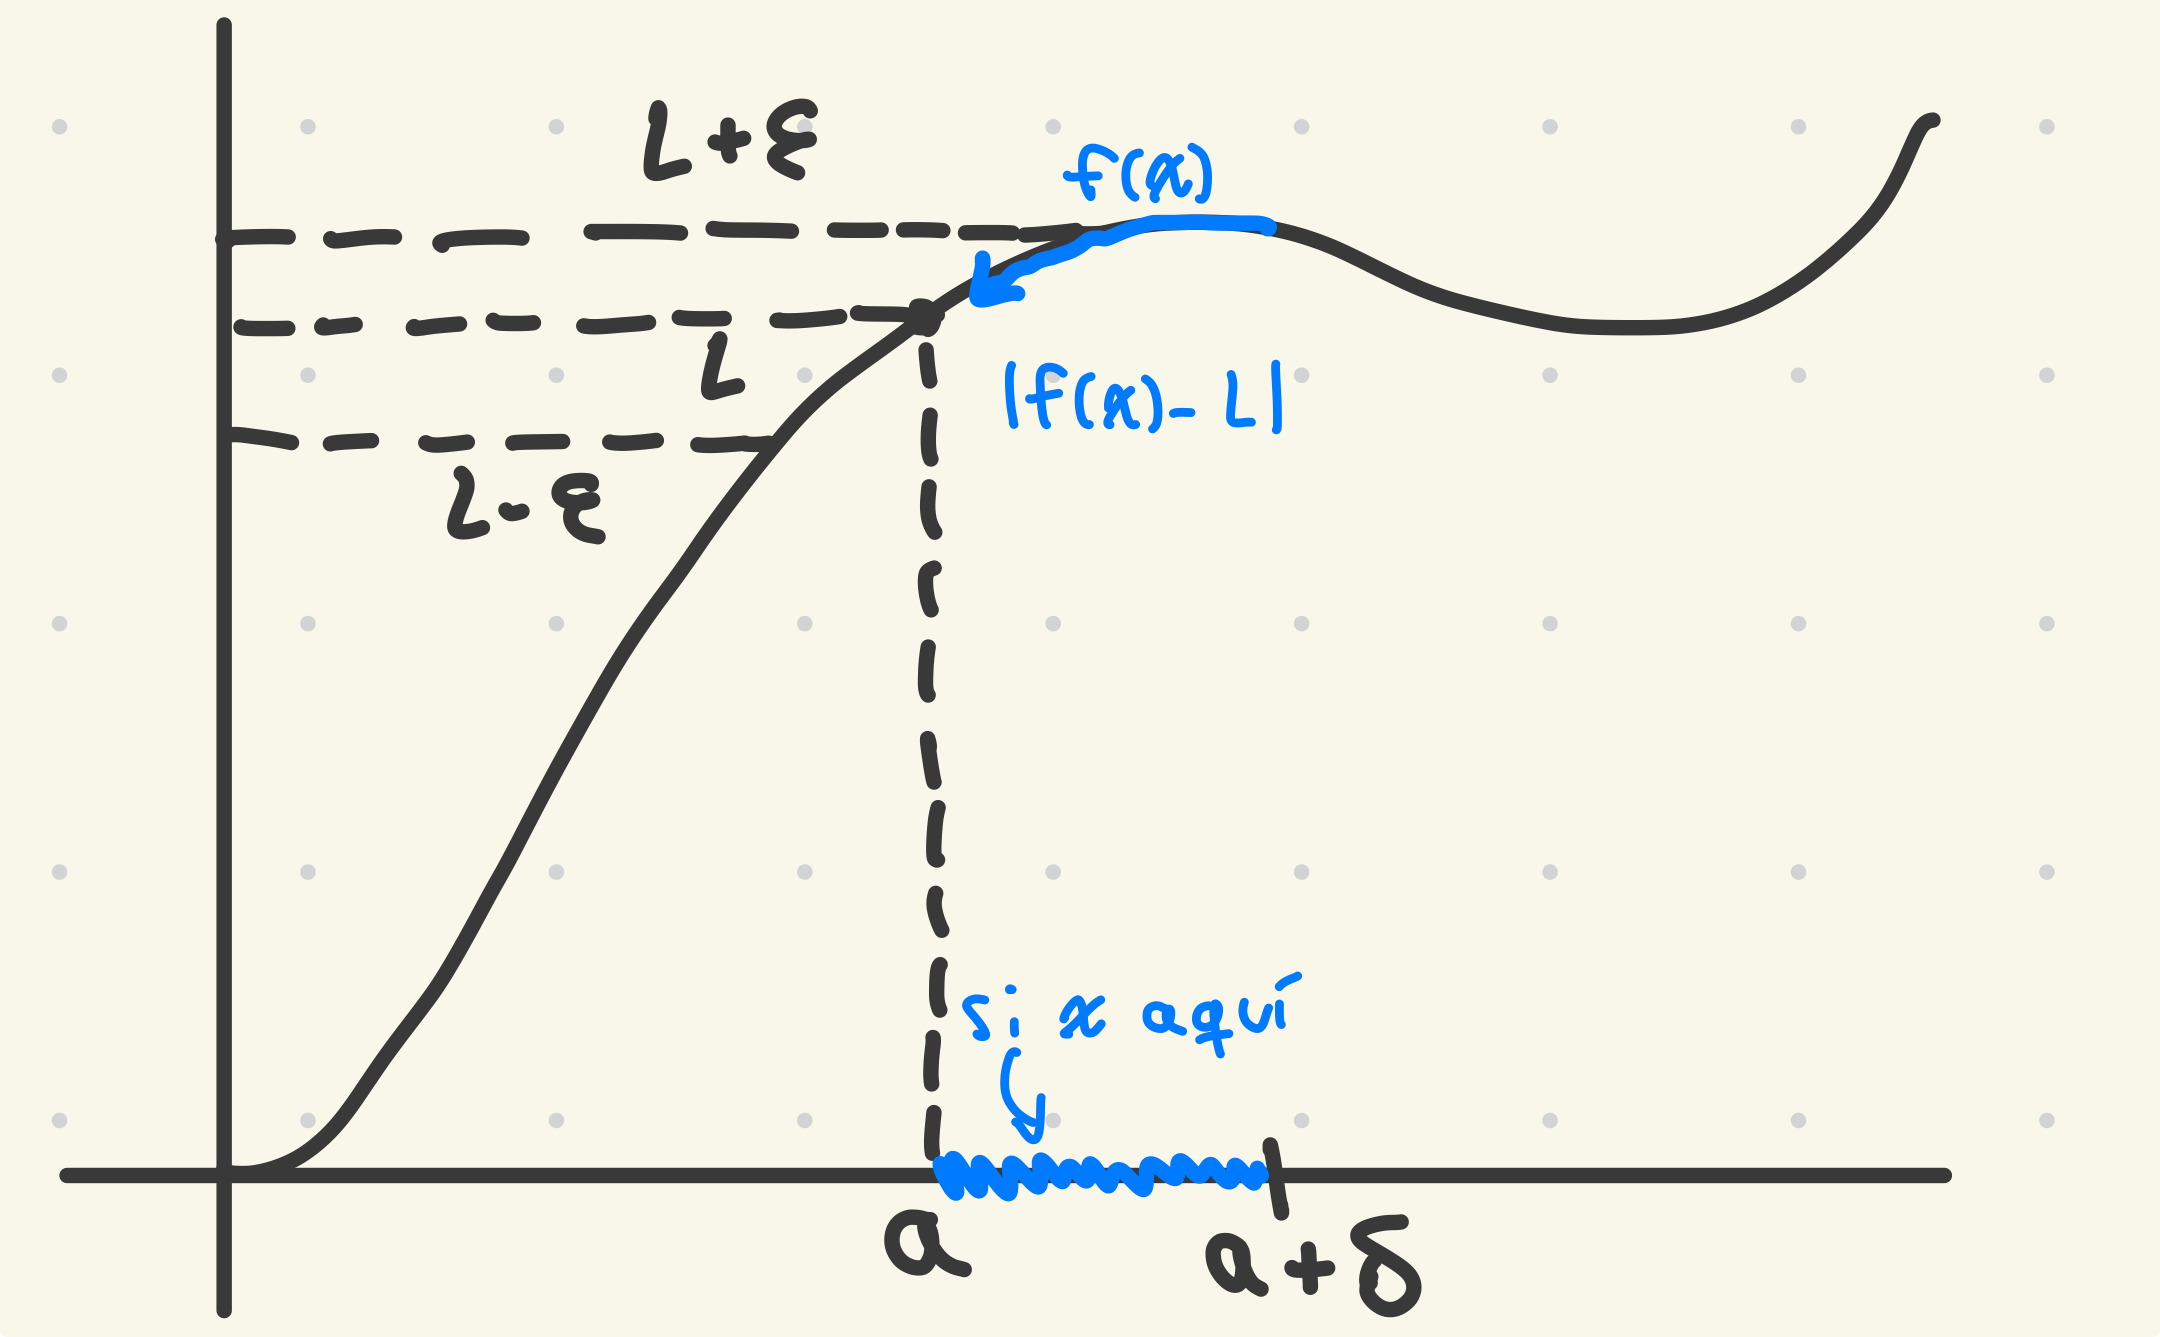
\includegraphics[height =100px]{limDerecha.jpg}
\end{center}
\begin{unicidad}[Teorema de unicidad del límite.]
    $\exists\lim_{x \to a} f(x)$ solo si existen ambos límites laterales y son iguales:
    \begin{equation}
        \begin{split}
            \lim_{x \to a^-} f(x)=\lim_{x \to a^+} f(x)
        \end{split}
    \end{equation}
    Además, el límite $l$ será
    \begin{equation}
        \begin{split}
            l = \lim_{x \to a} f(x)=\lim_{x \to a^-} f(x)=\lim_{x \to a^+} f(x)
        \end{split}
    \end{equation}
\end{unicidad}
\subsection{Propiedades de los límites}
Si tenemos dos funciones $f(x)$ y $g(x)$, y evaluamos el límite cuando ambas tienden al mismo valor $a$, entonces:\\
Sea $\lim_{x \to a}f(x)= m$ y $\lim_{x \to a}g(x)=n$:
\begin{itemize}
    \item $\lim_{x \to a} (f(x)+g(x))= m+n$
    \item $\lim_{x \to a} f(x) \cdot g(x)=m \cdot n$
    \item $\lim_{x \to a} \frac{1}{f(x)}= \frac{1}{m} / m \neq 0$
    \item $\lim_{x \to a} k ^{g(x)}= k^m$
    \item $\lim_{x \to a} f(x)^{g(x)}=\lim_{x \to a} f(x)^{\lim_{x \to a} g(x)}$
    \item $\lim_{x \to a} \log_k (g(x)) = \log_b(\lim_{x \to a}  (g(x)))$  
\end{itemize}
\section{Infinitesimales}
Una función es infinitesimal en $x=a$ si
\begin{equation}
    \begin{split}
        \lim_{x \to a}f(x)=0
    \end{split}
\end{equation}
\subsection{Infinitesimales comparables}
Sean dos funciones $f(x)$ y $g(x)$. Son infinitesimales comparables si
\begin{equation}
    \begin{split}
        \lim_{x \to a} \frac{f(x)}{g(x)} = k\;/\;k \in \mathbb{R}
    \end{split}
\end{equation}
Si
\begin{itemize}
    \item $k \neq 0$: $f(x)$ y $g(x)$ son infinitesimales de mismo orden
    cuando $x \to a$.
    \item $k = 0$ $f(x)$ es un infinitesimal de mayor orden que $g(x)$
    cuando $x \to a$.
\end{itemize}
\subsection{Infinitesimales equivalentes}
Si $f(x)$ y $g(x)$ son infinitesimales equivalentes, se verifica que
\begin{equation}
    \begin{split}
        \lim_{x \to a} \frac{f(x)}{g(x)} = 1 \implies f(x) \sim g(x)
    \end{split}
\end{equation}
\subsubsection{Lista de infinitesimales equivalentes}
\begin{equation}
    \begin{split}
        &x \to 0 \implies x \approx \sin x \approx \tan x \approx \arcsin x \approx \arctan x \approx
        \ln (1+x) \approx e^x -1\\
        &\frac{x^{2}}{2} \approx 1- \cos x
    \end{split}
\end{equation}
\begin{equation}
    \begin{split}
        f(x) \to 0 \implies f(x) \approx \ln (1 + f(x))
    \end{split}
\end{equation}
\begin{equation}
    \begin{split}
        f(x) \to 1 \implies \ln(f(x)) \approx f(x)-1
    \end{split}
\end{equation}
\section{Regla de comparaión de infinitos}
Se verifica que $\lim_{x \to a}f(x)= \pm \infty$ y $\lim_{x \to a} g(x)= \pm \infty$
\begin{enumerate}
    \item $f(x)$ es un infinito de orden superior a $g(x)$ si
    \begin{equation}
        \begin{split}
            \lim_{x \to a} \frac{f(x)}{g(x)} = \pm \infty
        \end{split}
    \end{equation}
    \item $f(x)$ es un infinito de orden inferior a $g(x)$ si
    \begin{equation}
        \begin{split}
            \lim_{x \to a} \frac{f(x)}{g(x)} = 0
        \end{split}
    \end{equation}
    \item $f(x)$ es un infinito de mismo orden que $g(x)$ si
    \begin{equation}
        \begin{split}
            \lim_{x \to a} \frac{f(x)}{g(x)} = k \quad / \quad k \in  \mathbb{R} - \{ 0 \}
        \end{split}
    \end{equation}
\end{enumerate}
\begin{sandwich}[Teorema del Sandwich]
    Sean tres funciones $f(x)$, $g(x)$ y $h(x)$.
    Si $\forall x \in (a,b) f(x) \leq g(x) \leq h(x)$ entonces:
    \begin{equation}
        \begin{split}
            \forall c \in (a,b) \lim_{x \to c} f(x) \leq
            \lim_{x \to c} g(x) \leq \lim_{x \to c} h(x)
        \end{split}
    \end{equation}
\end{sandwich}
\section{Continuidad}
Una función $f(x)$ es continua si:
\begin{equation}
    \begin{split}
        \forall \varepsilon > 0 \exists \delta > 0 / f(x_{0}) \in \mathbb{R} \implies 
        |x-x_{0}|-\delta  \implies |f(x)-f(x_{0})|<\varepsilon
    \end{split}
\end{equation}
Que verifica lo siguiente:
\begin{enumerate}
    \item $x_{0} \in Dom(f(x)) \implies f(x_{0}) \in \mathbb{R}$
    \item $\exists \lim_{x \to x_{0}^-} f(x) \wedge \exists \lim_{x \to x_{0}^+}f(x)$
    \item $\lim_{x \to x_{0}} f(x)=\lim_{x \to x_{0}^-} f(x)=\lim_{x \to x_{0}} f(x)=f(x_{0})$
\end{enumerate}
\begin{proof}[Teorema]
    Una función $f:\mathbb{D} \to \mathbb{R}$ es uniformemente continua en el subconjunto
    $E \subset D$ si y solo si
    \begin{equation}
        \begin{split}
            \forall \varepsilon > 0 \implies \exists \delta >0 / y \in E,
            |x-y|<\delta  \implies |f(x)-f(y)|<\varepsilon
        \end{split}
    \end{equation}
\end{proof}
\subsection{Continuidad lateral}
Por la izquierda (análogo a la derecha) se cumple:
\begin{enumerate}
    \item $x_{0} \in Dom(f)$
    \item $\exists \lim_{x \to x_{0}^{-}} f(x)$
    \item $f(x_{0})=\lim_{x \to x_{0}^{-}} f(x)$
\end{enumerate}
\subsection{Discontinuidades}
\subsubsection{Salto finito}
Se cumple si
\begin{equation}
    \begin{split}
        |\lim_{x \to x_{0}^{-}}-\lim_{x \to x_{0}^{+}}| \in \mathbb{R} -\{ 0 \}
    \end{split}
\end{equation}
\subsubsection{Salto infinito}
Se cumple si
\begin{equation}
    \begin{split}
        |\lim_{x \to x_{0}^{-}}-\lim_{x \to x_{0}^{+}}| \to \infty
    \end{split}
\end{equation}
\subsubsection{Evitable}
Se cumple cuando $\not \exists f(x_{0})$ pero sí $\lim_{x \to x_{0}}f(x)$
\end{document}
